\documentclass[tikz,border=10pt]{standalone}
\usetikzlibrary{positioning, arrows.meta}

\begin{document}
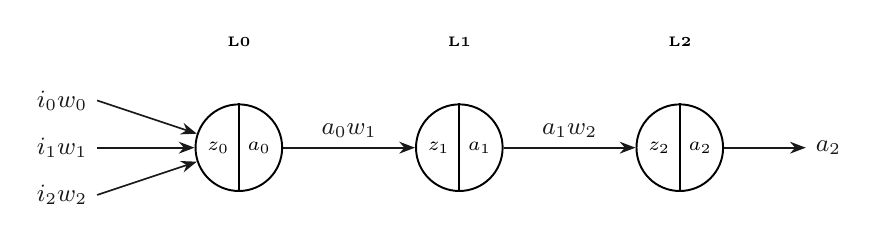
\begin{tikzpicture}[
    % Small, clean split neurons
    split_neuron/.style={circle, draw=black, minimum size=1.1cm, fill=white, line width=0.7pt},
    % Connection style
    connection/.style={-Stealth, line width=0.6pt, color=black!90}
]

    % --- LAYER 0 ---
    \node[split_neuron] (L0) at (0, 0) {};
    \draw[line width=0.7pt] (L0.north) -- (L0.south);
    \node at ([xshift=-0.26cm]L0.center) {\scriptsize $z_0$};
    \node at ([xshift=0.26cm]L0.center) {\scriptsize $a_0$};

    % --- INPUTS TO L0 ---
    \draw[connection] (-1.8, 0.6) -- (L0) node[pos=0, left] {\small $i_0 w_0$};
    \draw[connection] (-1.8, 0) -- (L0) node[pos=0, left] {\small $i_1 w_1$};
    \draw[connection] (-1.8, -0.6) -- (L0) node[pos=0, left] {\small $i_2 w_2$};

    % --- LAYER 1 ---
    \node[split_neuron] (L1) at (2.8, 0) {};
    \draw[line width=0.7pt] (L1.north) -- (L1.south);
    \node at ([xshift=-0.26cm]L1.center) {\scriptsize $z_1$};
    \node at ([xshift=0.26cm]L1.center) {\scriptsize $a_1$};

    % Connection L0 -> L1
    \draw[connection] (L0) -- (L1) node[midway, above, font=\small] {$a_0 w_1$};

    % --- LAYER 2 ---
    \node[split_neuron] (L2) at (5.6, 0) {};
    \draw[line width=0.7pt] (L2.north) -- (L2.south);
    \node at ([xshift=-0.26cm]L2.center) {\scriptsize $z_2$};
    \node at ([xshift=0.26cm]L2.center) {\scriptsize $a_2$};

    % Connection L1 -> L2
    \draw[connection] (L1) -- (L2) node[midway, above, font=\small] {$a_1 w_2$};

    % --- FINAL OUTPUT ---
    \draw[connection] (L2) -- (7.2, 0) node[right] {\small $a_2$};

    % --- COMPACT LAYER LABELS ---
    \node[above=0.6cm of L0, font=\tiny\bfseries] {L0};
    \node[above=0.6cm of L1, font=\tiny\bfseries] {L1};
    \node[above=0.6cm of L2, font=\tiny\bfseries] {L2};

\end{tikzpicture}
\end{document}
